\documentclass{article}
\usepackage[margin=2cm]{geometry}
\usepackage{float}
\usepackage{graphicx}

% Paragraph settings
\setlength{\parskip}{10pt plus 1pt minus 1pt
\setlength{\parindent}{0cm}}

\begin{document}
\title{Testing}
\author{Samuel Jackson \\ \texttt{slj11@aber.ac.uk}}
\date{\today}
\maketitle

\newpage
\section{Testing the Schedulers}
This document outlines the testing used with the scheduling algorithms in this assignment to ensure correct performance. To test the scheduler implementations a set of JUnit tests have been created and are available in a separate package called "Tests" located with the sources code. The rest of this document provides evidence of carrying out these tests on the algorithms.

\subsection{Shortest Time Remaining}
Shortest Time Remaining orders jobs according to the amount of processing they still need to do by when a job is added to the queue or and when it is returned to the scheduler after some processing. In the under lying code, both of these methods call the same method ($findPlace$) in order to place a job in the correct place on the queue. In order to test that the scheduler is working correctly I created JUnit tests that added the shortest job first, the shortest job second and two equally sized jobs to the queue. In each of these tests I then check that the correct job is returned from the $getNextJob$ method. I have also provided a test for the $returnJob$. As the code is almost identical underneath the hood as the $addNewJob$ I have only done a single test to check that a job that had a higher time remaining but now has a lower time remaining is moved further up the queue. Below is a screen image showing the the Shortest Time Remaining scheduler passing all JUnit tests.

\begin{figure}[H]
\centering
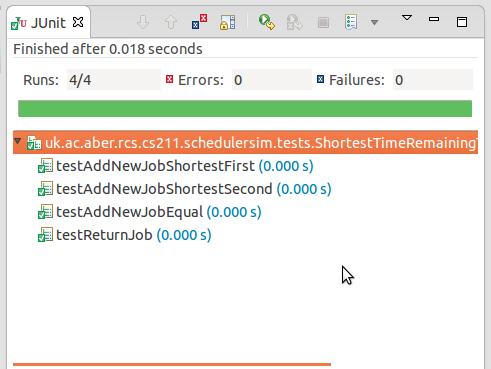
\includegraphics[width=0.5\textwidth]{img/str_test.png}
\caption{Shortest Time Remaining passing all JUnit tests.}
\label{fig:str-test}
\end{figure}

\subsection{Round Robin}
Round Robin orders jobs by taking the first job in the queue, performing some processing with it and then returning it to the back of the scheduler queue. Round Robin only uses the $returnJob$ method to order its jobs. In order to test that the scheduler works I created three tests each testing the scheduler with one, two and three jobs respectively. The following screen image shows all three of these tests passing.

\begin{figure}[H]
\centering
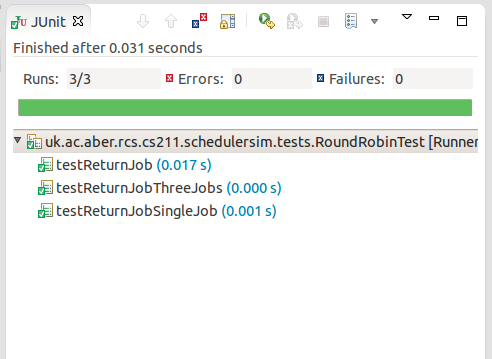
\includegraphics[width=0.5\textwidth]{img/rr_test.png}
\caption{Round Robin passing all JUnit tests.}
\label{fig:rr-test}
\end{figure}

\subsection{Lottery Scheduling}
Lottery Scheduling orders jobs according to a weight determined by the job's priority. Because the jobs are selected randomly testing lottery scheduling is more difficult than with the other two algorithms. In order to reliably generate the same sequence of random numbers for every test I used the exact same seed each time when setting up the test. This meant that the scheduler would produce repeatable output which could be measured against an expected criteria. To test this scheduler I carried out similar tests to each of the other algorithms such as testing the scheduler using one, two and three jobs when adding a new job and when returning a job to the scheduler. Below is a screen image showing the lottery scheduler class passing all tests.

\begin{figure}[H]
\centering
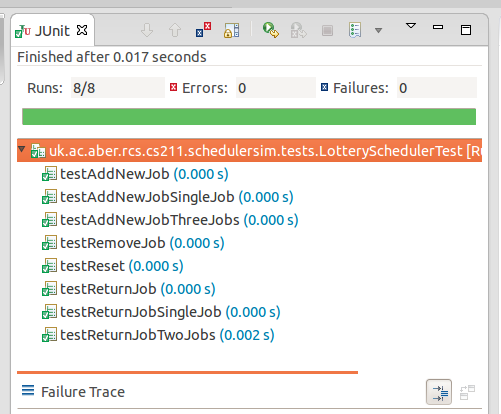
\includegraphics[width=0.5\textwidth]{img/lott_test.png}
\caption{Lottery Scheduling passing all JUnit tests.}
\label{fig:lott-test}
\end{figure}

\end{document}